\subsection{Mikrofonierung}
\notebox{Unter Mikrofonierung oder Mikrofonierungstechnik versteht man die situationsgerechte Auswahl und Aufstellung von geeigneten Mikrofonen zur Aufnahme von Schallquellen. Dabei bestimmen deren Richtcharakteristik und Frequenzgang die Einsatzgebiete. Je nach Aufstellungsort und Mikrofonanordnung sowie Zusammenmischung der Signale wird ein anderer Klang erzielt.\cite{dewiki:Mikrofonierung}}

Im groben sind für uns 3 Arten der Mikrofonierung relevant, die AB-, die XY- und die ORTF-Mikrofonierung. Dabei zu beachten ist das es noch weitere Arten der Aufnahmen gibt, diese 3 sind jedoch typische Vertreter. 

\begin{figure}[h]
    \centering
    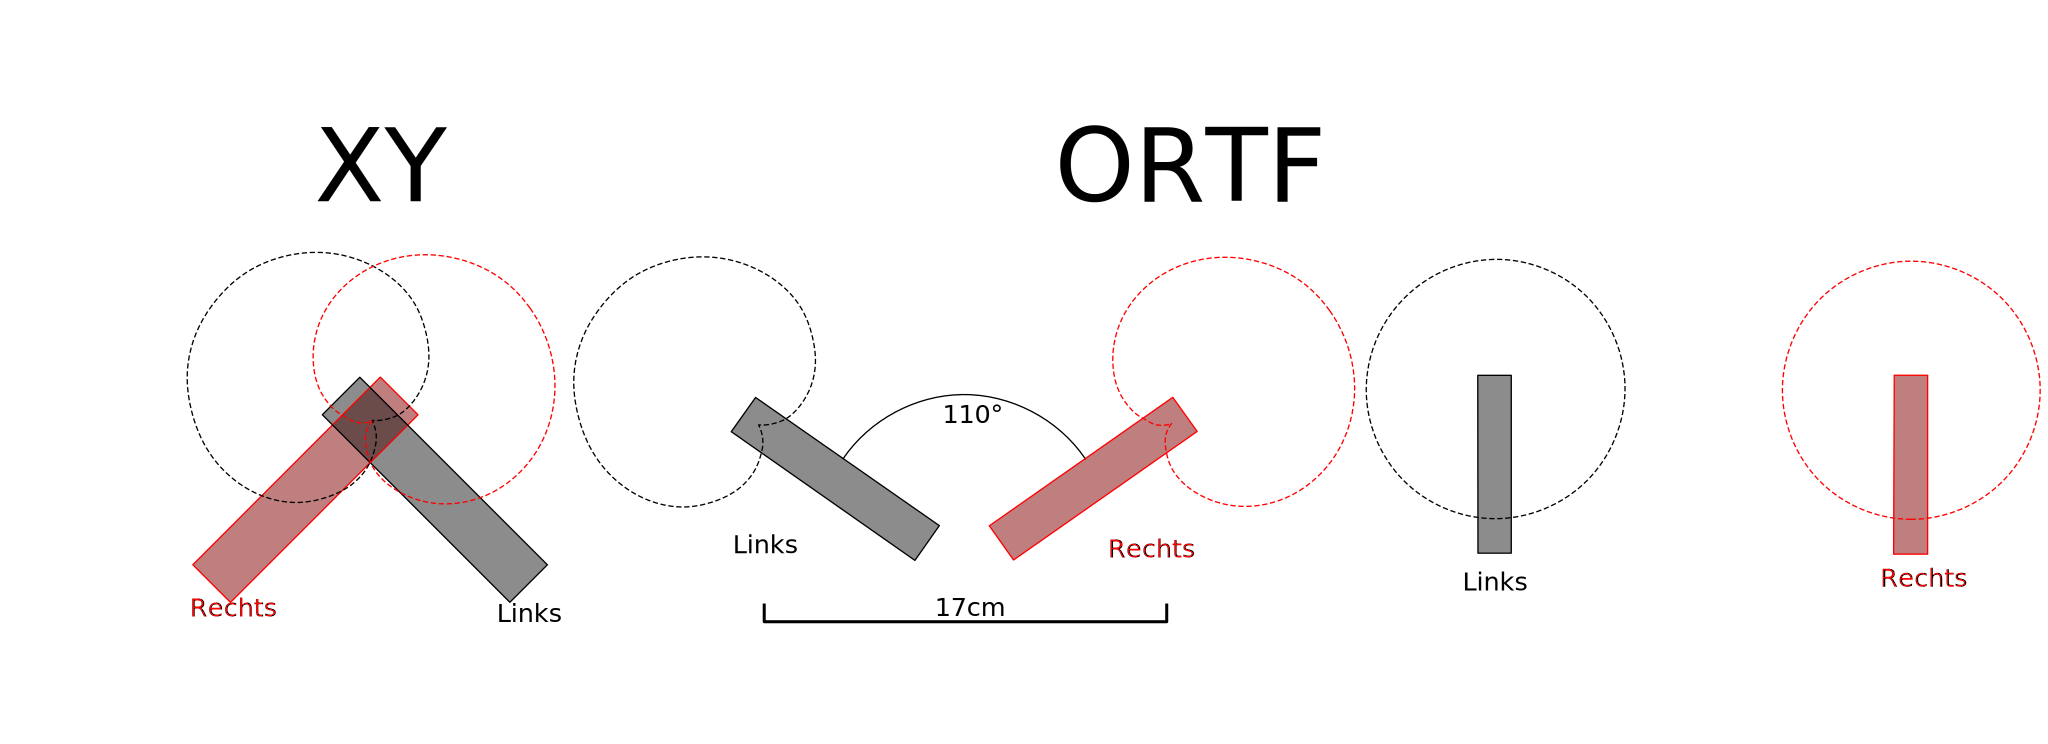
\includegraphics[width=1\linewidth]{Bilder/Medientechnik/Mikrofonierung.png}
    \caption{XY-, ORTF-, und AB-Mikrofonierung}
    \label{fig:Mikrofonierung}
\end{figure}
\newpage


